%% ICDCN 2027 poster track: 2-page extended abstract, ACM sigconf (acmart v2.20).
%% Generated into abstract.tex by `python -m traffic.abstract_build`; edit this
%% template, not abstract.tex. Double-angle-bracket fields are filled from outputs/.
\documentclass[sigconf]{acmart}

%% Review submission: no rights block or ACM reference box. For camera-ready, replace
%% these two lines with the rights commands ACM sends after the eRights form.
\setcopyright{none}
\settopmatter{printacmref=false}
\renewcommand\footnotetextcopyrightpermission[1]{}

\acmConference[ICDCN 2027]{28th International Conference on Distributed Computing and Networking}{January 4--7, 2027}{Mangaluru, India}

\usepackage{booktabs}

\begin{document}

\title{Plan for the Ground You Will Drive On: Forecast-Aware Off-Road Route Planning on the Vehicle}

%% Single-blind review: real names, affiliations and emails go here.
\author{[Author One]}
\affiliation{\institution{[Institution]}\city{[City]}\country{India}}
\email{[author.one@institution.edu]}
\author{[Author Two]}
\affiliation{\institution{[Institution]}\city{[City]}\country{India}}
\email{[author.two@institution.edu]}

\begin{abstract}
Off-road trafficability changes from day to day: a monsoon week can turn firm ground to
mud, so a route that is passable when it is planned may not be when it is driven. Forward
units also cannot count on a weather service or a network link. We forecast ground
firmness one to seven days ahead on the vehicle, from a local weather log (GRU and ridge
regression, 531k parameters, 12\,ms per forecast on one CPU core), turn it into
per-vehicle NO-GO maps with a fuzzy AND of slope, land cover and soil, and plan for the day
of travel. A convoy shares only its tracks, so each vehicle accounts for ground churned by
those ahead. In a backtest of 325,800 trips over two monsoons on the Pachmarhi plateau,
planning three days ahead on the forecast sent 24\% fewer trips into mud than planning
on today's map, and at equal risk held back 31--40\% fewer trips than a safety margin
on today's map.
\end{abstract}

\begin{CCSXML}
<ccs2012>
<concept><concept_id>10010520.10010553</concept_id>
<concept_desc>Computer systems organization~Embedded and cyber-physical systems</concept_desc>
<concept_significance>500</concept_significance></concept>
<concept><concept_id>10010147.10010257.10010293.10010294</concept_id>
<concept_desc>Computing methodologies~Neural networks</concept_desc>
<concept_significance>300</concept_significance></concept>
</ccs2012>
\end{CCSXML}
\ccsdesc[500]{Computer systems organization~Embedded and cyber-physical systems}
\ccsdesc[300]{Computing methodologies~Neural networks}

\keywords{edge computing, trafficability, route planning, soil strength forecasting, convoy coordination}

\maketitle

\section{Problem}
Off the road, the soil decides which vehicles move. The NATO Reference Mobility Model
rates soil strength as a rating cone index (RCI) and each vehicle by a vehicle cone index:
a vehicle is stuck on the first pass where RCI\,$<$\,VCI$_1$ and can sustain traffic where
RCI\,$\geq$\,VCI$_{50}$~\cite{rosca2018}. Dynamic trafficability maps combine terrain and
weather factors for the time they are built~\cite{liu2025}. Two things are missing. The
ground on the day of travel differs from the day of planning, and forward units planning
off the network have no weather service to ask. We test whether a forecast small enough to
run on the vehicle produces better routes, and what a convoy must exchange to plan together.

\section{System}
\textbf{Ground firmness.} The site is the Pachmarhi plateau (Satpura range, 1,067\,m), with
a daily record for 2015--2025 (4,018 days): ERA5-Land soil moisture in two
layers~\cite{munoz2021} and IMD rainfall (ERA5 for 2025). With each layer scaled to its 11-year range,
$\mathrm{SWI}=0.35\,s_{0\text{--}7}+0.65\,s_{7\text{--}28}$ and
$\mathrm{RCI}=300\,e^{-3.0\,\mathrm{SWI}}\,(1-0.15\min(R_{3d}/50\,\mathrm{mm},1))$\,psi, where
$R_{3d}$ is the last three days' rain. The saturated value, 15\,psi, follows field readings
on lanes where a 4$\times$4 bogged down~\cite{rosca2018}.

\textbf{Vehicles.} From a public 2,451-row vehicle-attribute list we keep 1,145 ground
vehicles (1,004 tracked, 125 wheeled, 16 half-tracks). Each gets VCI$_1$
and VCI$_{50}$ from the Mobility Index~\cite{rosca2018,ciobotaru2009}, with running gear
assumed by weight class. Our tracked implementation reproduces the published M1 example
(MI 98.6, VCI$_1$ 26.3). Results are reported for five VCI$_1$ bands, which are NO-GO on
10--30\% of days.

\textbf{Edge forecaster.} A GRU (128$\times$2)~\cite{cho2014} and a ridge regression,
averaged, predict the change in RCI 1--7 days ahead from 60 days of local history, with no
numerical weather prediction. A safety margin per band is subtracted before the comparison
with VCI$_1$. Each margin is tuned to catch 90\% of NO-GO days on one test year and scored
on the other.

\textbf{Maps and planning.} The plateau-wide RCI is spread over a 90\,m grid
(76k cells) by topographic wetness index~\cite{beven1979}, shifting each cell's SWI by
up to $\pm$0.2. Terrain comes from a Google Earth Engine export (DEM, ESA
WorldCover~\cite{zanaga2022}, Sentinel-2 NDVI as canopy density) and 403 OpenStreetMap
road segments~\cite{osm}. Slope and land-cover memberships follow Liu et al.'s
tables~\cite{liu2025}. Soil membership is 0 below VCI$_1$ and rises to 1 at VCI$_{50}$, so
SLOW-GO is slow, not forbidden. Cells combine by fuzzy AND (minimum)~\cite{zadeh1965},
which vetoes deal-breakers by construction. Routes minimise travel time with speed
proportional to membership (Dijkstra, equivalent to A*).

\textbf{Convoys.} Each pass raises the firmness the next vehicle needs, which we model as
$\mathrm{VCI}(n)=\mathrm{VCI}_1+(\mathrm{VCI}_{50}-\mathrm{VCI}_1)\ln n/\ln 50$. In the
wear-aware mode each vehicle broadcasts its track (4\,B per cell), and the next one plans
on the shared pass-count map.

\section{Evaluation}
\textbf{Forecast.} Over the 2024--25 test years, the 7-day RMSE is 20.8\,psi against
26.0 for persistence (20\% lower). At 90\% NO-GO recall the forecast makes
23--45\% fewer false NO-GO calls per vehicle-year than the same margin rule
applied to today's value.

\begin{figure}[t]
  \centering
  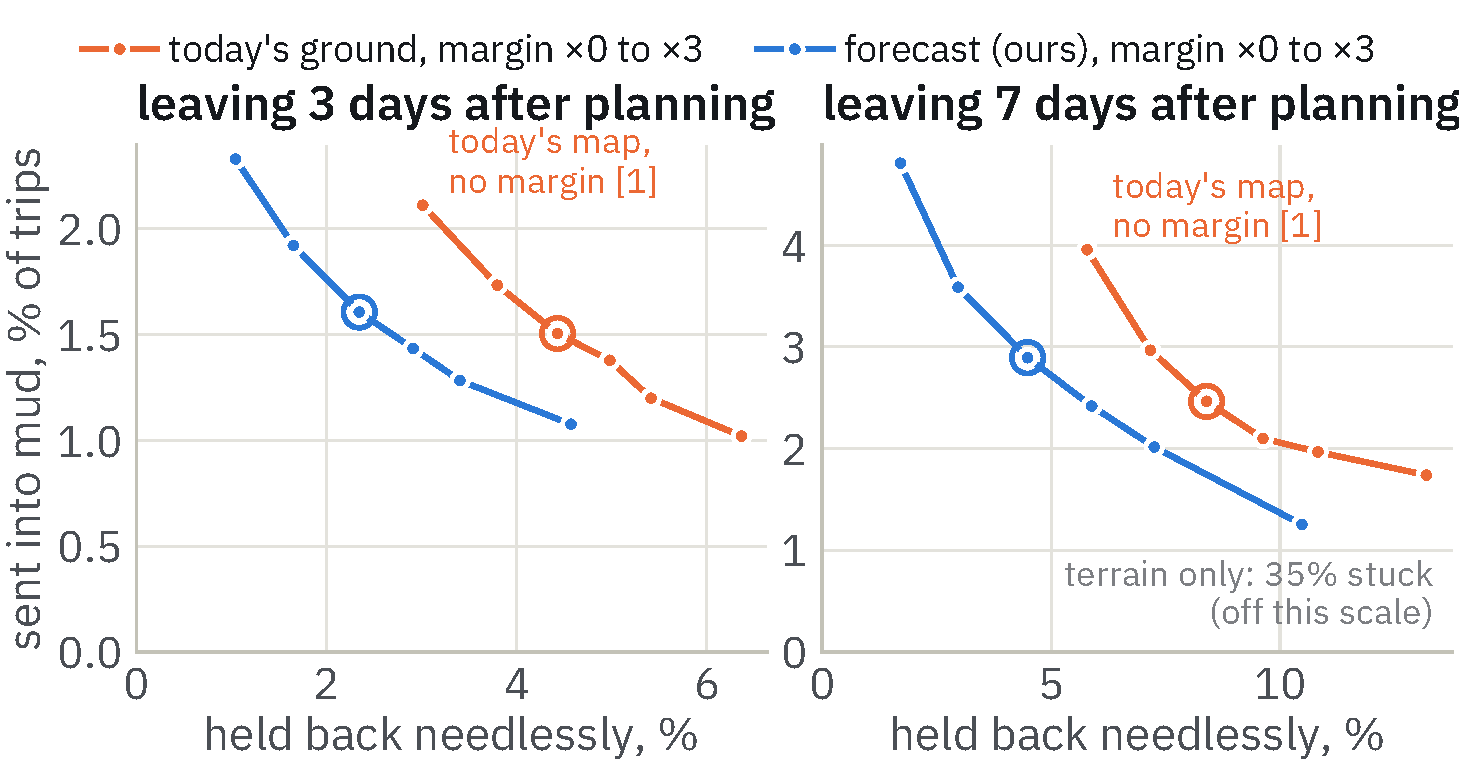
\includegraphics[width=\columnwidth]{figures/f5_tradeoff.pdf}
  \caption{Both planning errors as each planner's safety margin goes from none to
  $3\times$ the tuned value (ringed). Lower left is better.}
  \label{fig:tradeoff}
\end{figure}

\textbf{Routing backtest.} For every test day, band and lead time $h\in\{1,3,7\}$ we plan 30
trips of 8--25\,km between points on the road network and score each plan against the real
ground on the day of travel. A plan is \emph{stuck} if its route crosses a NO-GO cell and
\emph{held} if it finds no route when one existed (Table~\ref{tab:bt}). Planning on the
forecast beats today's map on both errors: 1.6\% against 2.1\% stuck at 3 days
($-$24\%) and 2.9\% against 3.9\% at 7 days ($-$26\%), with fewer
trips held back. A margin on today's value is slightly safer at its tuned setting but holds
back far more trips. Sweeping both margins (Fig.~\ref{fig:tradeoff}) shows the forecast
dominating: at an equal stuck rate it holds back 40\% (3 days) and 31\% (7
days) fewer trips. Extra travel time against the best route is under 0.1\%. A weighted mean
of factor scores without a veto sends 34.8\% of trips into mud; with Liu et al.'s veto,
1.8\%. No model foresees the day the monsoon breaks without a weather forecast; the gain
comes in the days around the transitions.

\begin{table}[t]
  \caption{Routing backtest, 2024--25: share of trips sent into mud (stuck) and of possible
  trips held back, by planner and lead time.}
  \label{tab:bt}
  \small
  \begin{tabular}{@{}lrrrr@{}}
    \toprule
    & \multicolumn{2}{c}{3 days} & \multicolumn{2}{c}{7 days} \\
    Planner & stuck & held & stuck & held \\
    \midrule
    Terrain only            & 35.5\% & 0.0\% & 35.5\% & 0.0\% \\
    Today's map~\cite{liu2025} & 2.1\% & 3.0\% & 3.9\% & 5.8\% \\
    Today + margin          & 1.5\% & 4.4\% & 2.5\% & 8.4\% \\
    \textbf{Forecast + margin} & \textbf{1.6\%} & \textbf{2.3\%} & \textbf{2.9\%} & \textbf{4.4\%} \\
    \bottomrule
  \end{tabular}
\end{table}

\begin{figure}[t]
  \centering
  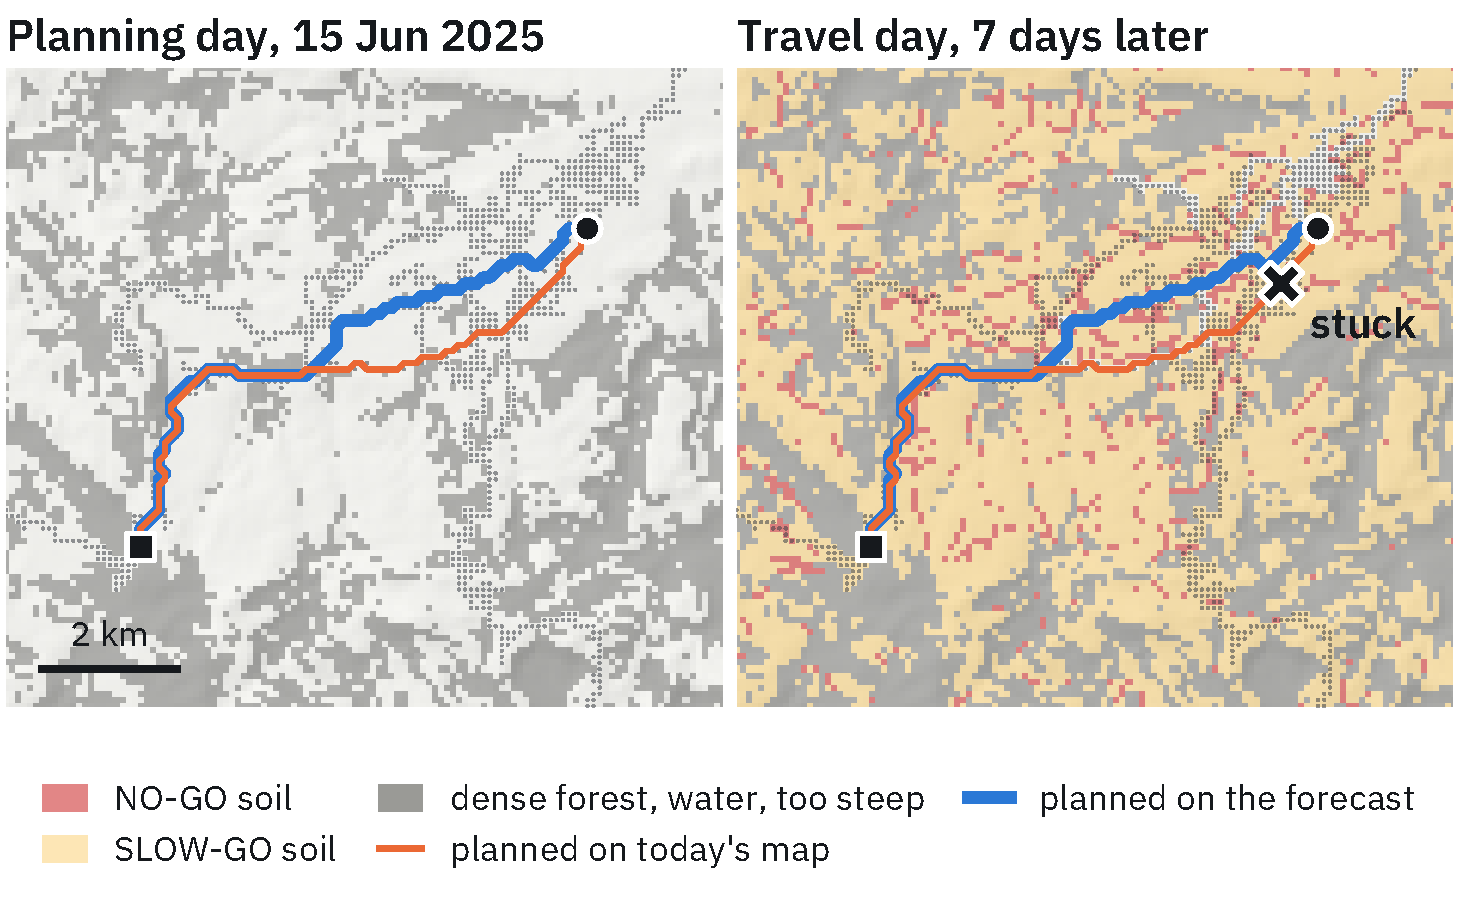
\includegraphics[width=\columnwidth]{figures/f4_map.pdf}
  \caption{One trip from the backtest. Planned on 15 June 2025 for 7 days later, the route on
  today's map (orange) crosses ground that is NO-GO by the travel day ($\times$); the route
  planned on the forecast (blue) avoids it.}
  \label{fig:map}
\end{figure}

\textbf{Convoys and the network.} On 54 soft days, ten heavy tracked vehicles that
follow the leader get 5.5 through on average; re-planning on the shared pass-count
map gets 9.2 through, for 6.9\,kB of track updates per convoy. Wheeled vehicles
gain less (6.4 to 7.0) because the forest leaves them few parallel lanes. A
7-day forecast is 18\,B, against 76\,kB for one passability map, so the link
carries 4,200$\times$ less when vehicles rebuild maps locally. The model is
2.0\,MB, and re-planning a route takes 25\,ms.

\section{Limitations and Next Steps}
RCI is computed from modelled soil moisture in one 9\,km cell, not measured, and spreading
it by wetness index has no field check. Vehicle masses come from a game-file dataset, with
wheeled masses corrected from open sources, so we report bands rather than named vehicles.
Tuned margins differ between the two test years by up to 7.2\,psi. Next:
cone-penetrometer readings at Pachmarhi, Sentinel-1 radar as a soil-moisture input,
persistent ruts, and convoy trials over real tactical radio links.

\bibliographystyle{ACM-Reference-Format}
\bibliography{refs}

\end{document}
